\chapter{Introduction, Threat Modeling, and Security Objectives}
\label{chap:intro}

This chapter delineates the operational context of cloud-native enterprise Artificial Intelligence (AI) services, formalizes the threat landscape regarding computational resource exhaustion (Semantic DoS), and defines the fundamental security objectives enforced by the proposed architecture.

\section{The Landscape of Enterprise Cloud AI Applications}
Integrating Large Language Models (LLMs) and deep neural network inference into mission-critical corporate workflows has reshaped cloud service topologies. Unlike standard microservices where request latency is bounded in tens of milliseconds with nominal CPU usage, generative AI endpoints feature an acute computational asymmetry:
\begin{itemize}
    \item \textbf{Rapid VRAM and Memory Footprint}: Model parameter loading and context window allocation instantaneously allocate gigabytes of high-bandwidth memory (GPU VRAM / host RAM).
    \item \textbf{Intensive Matrix Computations}: Autoregressive token generation continuously monopolizes matrix compute units (Tensor Cores) for the entire duration of the streaming response.
    \item \textbf{KV-Cache Persistence}: Holding self-attention Key-Value (KV) cache states across concurrent user sessions binds backend system resources for extended intervals.
\end{itemize}

An unauthenticated remote adversary transmitting high-frequency sub-kilobyte requests can exhaust server computational capacity without generating significant network bandwidth, rendering traditional network-layer bandwidth filters insufficient.

\section{Threat Modeling Matrix}
To systematically categorize incoming threats, we define a multi-dimensional threat matrix targeting the ingress-to-backend continuum (Figure~\ref{fig:threat_matrix}):

\begin{figure}[htbp]
\centering
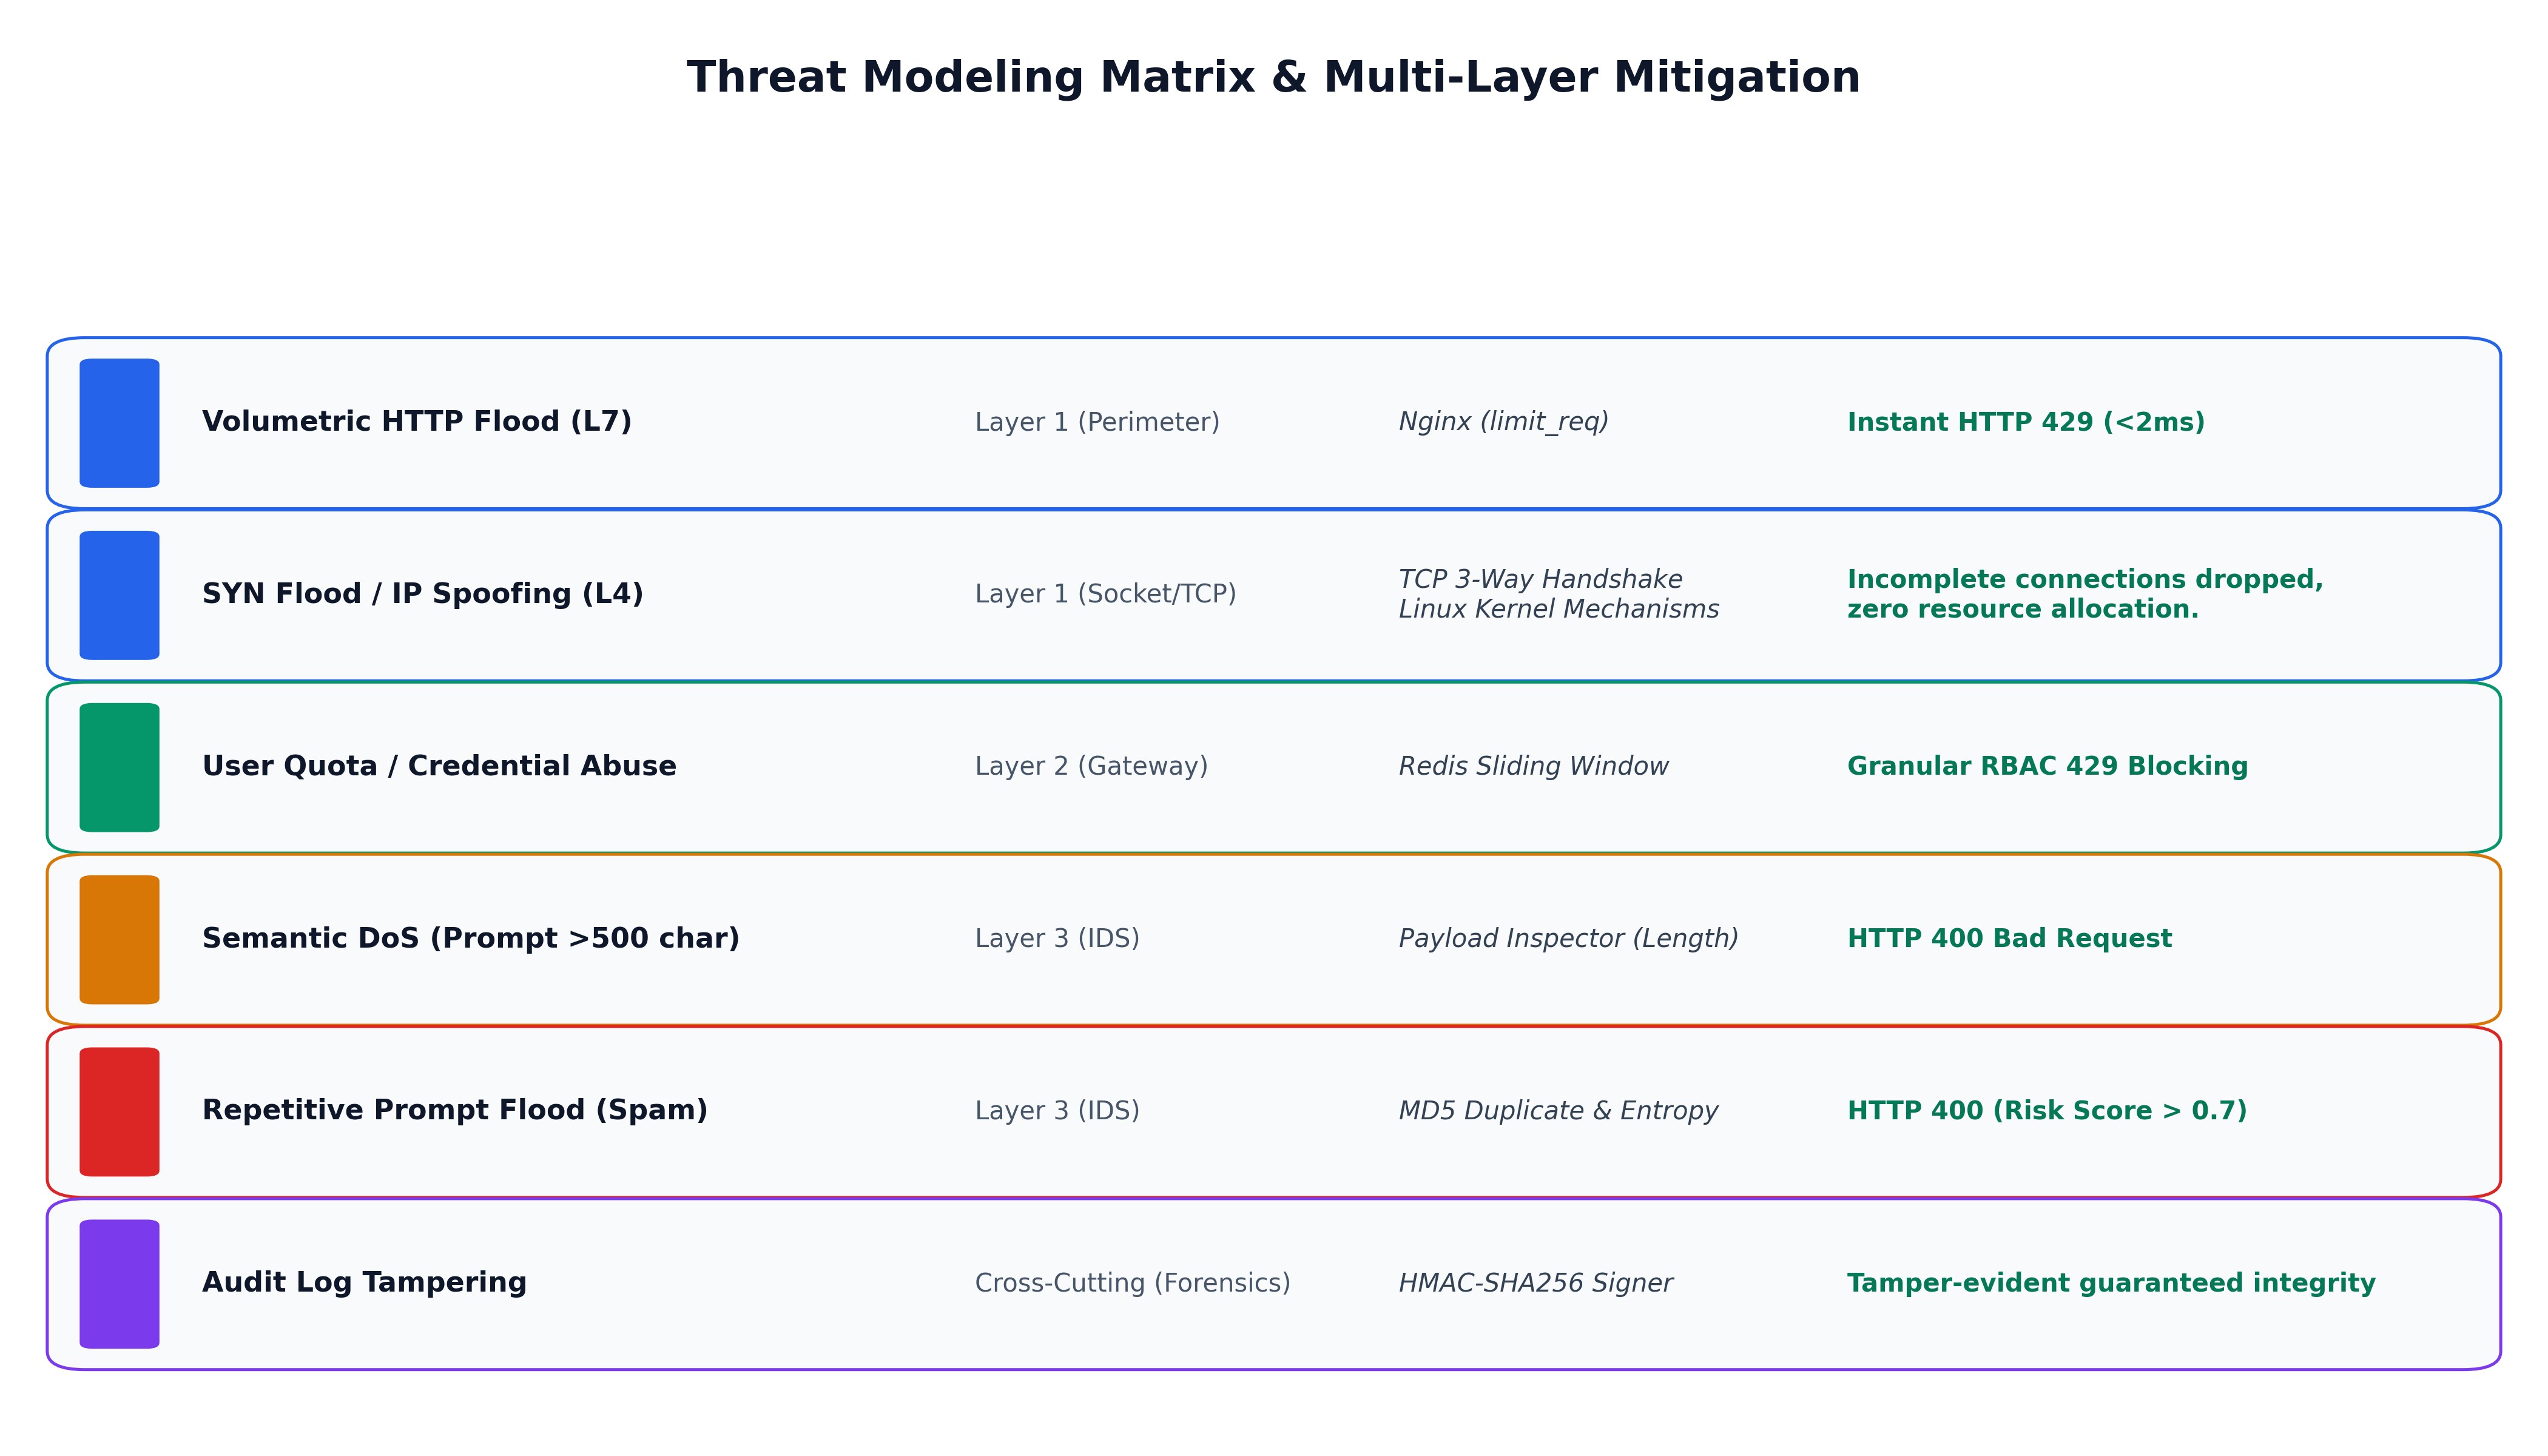
\includegraphics[width=0.95\textwidth]{figures/threat_model_mitigation.png}
\caption{Threat Modeling Matrix and Corresponding Multi-Layer Mitigation Strategy.}
\label{fig:threat_matrix}
\end{figure}

The threat categories addressed include:
\begin{enumerate}
    \item \textbf{Layer 4/Layer 7 Volumetric HTTP Flood}: High-concurrency socket floods designed to overwhelm socket descriptors and concurrency thread pools.
    \item \textbf{Credential and Quota Abuse}: Exploitation of unmetered API endpoints or unauthorized access via forged or missing tokens.
    \item \textbf{Semantic DoS via Oversized Prompts}: Prompts exceeding nominal input lengths intended to force quadratic memory expansion in self-attention mechanisms ($O(N^2)$ complexity).
    \item \textbf{Repetitive Token Spamming}: Highly redundant repetitive strings designed to invoke pathological worst-case decoding behaviors while remaining syntactically valid JSON.
    \item \textbf{Forensic Tampering}: Illegitimate alteration of audit and access logs to obscure intrusion attempts.
\end{enumerate}

\section{Security Objectives and Defense-in-Depth Principle}
The primary objective of the \textbf{C-DIDA} architecture is to enforce strict adherence to the \textit{Defense-in-Depth} paradigm (NIST SP 800-207 Zero Trust Architecture \cite{nist_800_207}). Every transaction must pass through progressively deeper inspection gates:
\begin{itemize}
    \item \textbf{Early Rejection}: Inadmissible requests must be terminated as close to the network perimeter as possible, minimizing CPU time spent on unauthenticated traffic.
    \item \textbf{Zero Unauthenticated Computation}: The inference engine must never process payloads that have not passed cryptographic signature verification and structural sanity checks.
    \item \textbf{Auditability}: Every policy violation must generate an immutable, tamper-evident forensic log.
\end{itemize}
